\documentclass{article}
\usepackage[utf8]{inputenc}
\usepackage{amsmath}
\usepackage{amssymb}
\usepackage{float}
\usepackage{framed}
\usepackage{pgfplots}
\usepackage{tikz}
\usepackage{relsize}
\usepackage{hyperref}
\usepackage{subfiles}
\pgfplotsset{compat=newest}
\title{%
    ECN 1101 - Introductory Maths - Semester 1 2021 \\
    \large Worksheet 3 \\
}
\author{Lecturer: Anand Persaud \\ "Transliterator": Simeon Chester \\}
\date{2021-11-07}
\begin{document}
\maketitle
\relscale{1.5}

\textbf{This worksheet accompanies lecture notes 1 on straight line geometry/coordinate geometry}

\section{For each of the following points find:}
\begin{description}
    \item[a.] the midpoint
    \item[b.] the length of the line
    \item[c.]  the equation of the line
        \clearpage
        \subsection{(-2, 10),(5, 3)}
        \label{subsection:1.1}
        \underline{MIDPOINT}
        $$
            \begin{aligned}
                midpoint & = (\frac{x_1+x_2}{2}, \frac{y_1+y_2}{2}) \\
                         & = (\frac{-2+5}{2}, \frac{10+3}{2})       \\
                         & = (\frac{3}{2}, \frac{13}{2})            \\
                         & = (1.5, 6.5)                             \\
            \end{aligned}
        $$

        \underline{LENGTH OF LINE}
        $$
            \begin{aligned}
                length \ of \ line & = \sqrt{(x_2-x_1)^2 + (y_2-y_1)^2} \\
                                   & = \sqrt{(5-(-2))^2 + (3-10)^2}     \\
                                   & = \sqrt{(7)^2 + (-7)^2}            \\
                                   & = \sqrt{49 + 49}                   \\
                                   & = \sqrt{98}                        \\
                                   & = 9.90                             \\
            \end{aligned}
        $$

        \underline{SLOPE OF LINE}
        $$
            \begin{aligned}
                m & = \frac{y_2-y_1}{x_2-x_1} \\
                  & = \frac{3-10}{5-(-2)}     \\
                  & = \frac{-7}{7}            \\
                  & = -1.00                   \\
            \end{aligned}
        $$

        \underline{EQUATION OF THE LINE}

        Using the points $(-2, 10)$ and $m=-1$ we find $c$
        $$
            \begin{aligned}
                y & = mx + c        \\
                c & = y - mx        \\
                c & = 10 - (-1)(-2) \\
                c & = 10 - 2        \\
                c & = 8             \\
            \end{aligned}
        $$
        Therefore the equation is
        $$
            y = -x + 8
        $$
        \begin{figure}[H]
            \begin{center}
                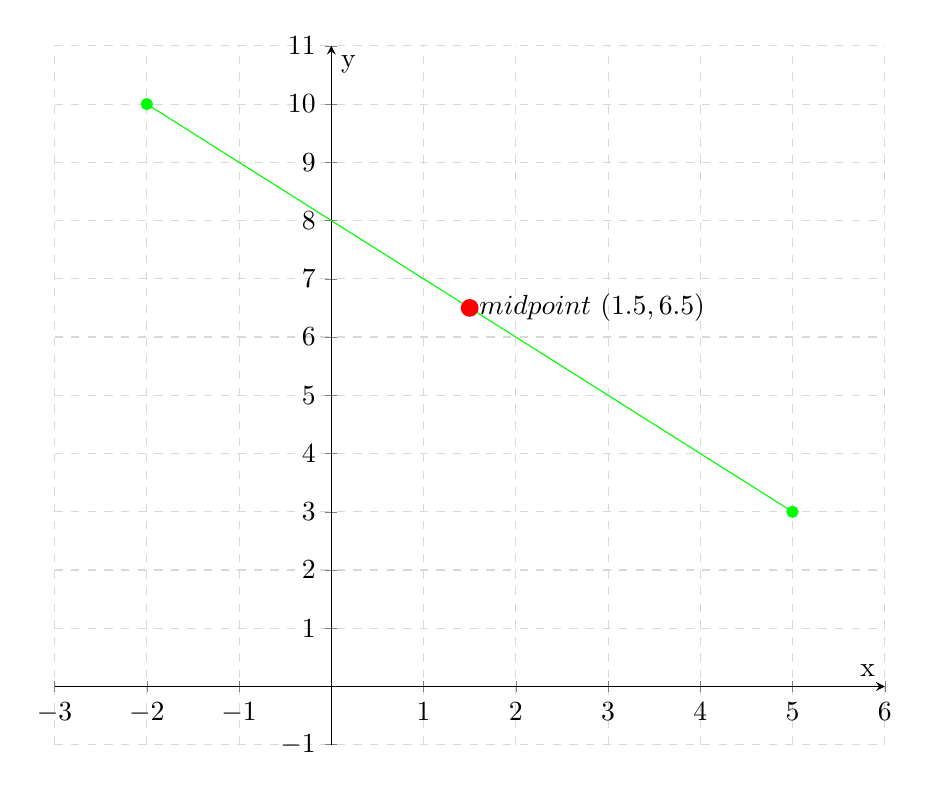
\begin{tikzpicture}
                    \begin{axis}[
                            width= \linewidth,
                            xmin = -3,
                            xmax = 6,
                            ymin=-1,
                            ymax=11,
                            ytick={-1,0,1,2,3,4,5,6,7,8,9, 10,11},
                            xlabel=x,
                            ylabel=y,
                            grid=major,
                            grid style = {dashed, gray!30},
                            axis lines = center,
                            clip = false
                        ]

                        \addplot[color=green,mark=*] coordinates {
                                (-2, 10)
                                (5, 3)
                            };

                        \addplot[color=red, mark=*, mark size=3pt] coordinates {
                                (1.5, 6.5)
                            };

                        \node [right] at (axis cs: 1.5, 6.5) {$midpoint \ (1.5, 6.5)$};

                    \end{axis}
                \end{tikzpicture}
                \caption{\label{Graph-1}Graph showing $y=-x+8$}
            \end{center}
        \end{figure}
        \clearpage
        \subsection{(6, -2),(8, -3)}
        \underline{MIDPOINT}
        $$
            \begin{aligned}
                midpoint & = (\frac{x_1+x_2}{2}, \frac{y_1+y_2}{2}) \\
                         & = (\frac{6+8}{2}, \frac{-2-3}{2})        \\
                         & = (\frac{14}{2}, \frac{-5}{2})           \\
                         & = (7, -2.5)                              \\
            \end{aligned}
        $$

        \underline{LENGTH OF LINE}
        $$
            \begin{aligned}
                length \ of \ line & = \sqrt{(x_2-x_1)^2 + (y_2-y_1)^2} \\
                                   & = \sqrt{(8-6)^2 + (-3-(-2))^2}     \\
                                   & = \sqrt{(2)^2 + (-1)^2}            \\
                                   & = \sqrt{4 + 1}                     \\
                                   & = \sqrt{5}                         \\
                                   & = 2.24                             \\
            \end{aligned}
        $$

        \underline{SLOPE OF LINE}
        $$
            \begin{aligned}
                m & = \frac{y_2-y_1}{x_2-x_1} \\
                  & = \frac{-3-(-2)}{8-6}     \\
                  & = \frac{-1}{2}            \\
                  & = -0.5                    \\
            \end{aligned}
        $$

        \underline{EQUATION OF THE LINE}

        Using the points $(6, -2)$ and $m=-0.5$ we find $c$
        $$
            \begin{aligned}
                y & = mx + c         \\
                c & = y - mx         \\
                c & = -2 - (-0.5)(6) \\
                c & = -2+3           \\
                c & = 1              \\
            \end{aligned}
        $$
        Therefore the equation is
        $$
            y = -0.5x+1
        $$
        \begin{figure}[H]
            \begin{center}
                \begin{tikzpicture}
                    \begin{axis}[
                            width= \linewidth,
                            xmin = 5,
                            xmax = 9,
                            ymin=-4,
                            ymax=0,
                            xlabel=x,
                            ylabel=y,
                            grid=major,
                            grid style = {dashed, gray!30},
                            axis lines = center,
                            clip = false
                        ]

                        \addplot[color=green,mark=*] coordinates {
                                (6, -2)
                                (8, -3)
                            };

                        \addplot[color=red, mark=*, mark size=3pt] coordinates {
                                (7, -2.5)
                            };

                        \node [right] at (axis cs: 7, -2.5) {$midpoint \ (7, -2.5)$};

                    \end{axis}
                \end{tikzpicture}
                \caption{\label{Graph-2}Graph showing $y=-0.5x+1$}
            \end{center}
        \end{figure}
        \clearpage
        \subsection{(0, -6),(3, 0)}
        \underline{MIDPOINT}
        $$
            \begin{aligned}
                midpoint & = (\frac{x_1+x_2}{2}, \frac{y_1+y_2}{2}) \\
                         & = (\frac{0+3}{2}, \frac{-6+0}{2})        \\
                         & = (\frac{3}{2}, \frac{-6}{2})            \\
                         & = (1.5, -3)                              \\
            \end{aligned}
        $$

        \underline{LENGTH OF LINE}
        $$
            \begin{aligned}
                length \ of \ line & = \sqrt{(x_2-x_1)^2 + (y_2-y_1)^2} \\
                                   & = \sqrt{(3-0)^2 + (0-(-6))^2}      \\
                                   & = \sqrt{(3)^2 + (6)^2}             \\
                                   & = \sqrt{9 + 36}                    \\
                                   & = \sqrt{45}                        \\
                                   & = 6.71                             \\
            \end{aligned}
        $$

        \underline{SLOPE OF LINE}
        $$
            \begin{aligned}
                m & = \frac{y_2-y_1}{x_2-x_1} \\
                  & = \frac{0-(-6)}{3-0}      \\
                  & = \frac{6}{3}             \\
                  & = 2                       \\
            \end{aligned}
        $$

        \underline{EQUATION OF THE LINE}

        Using the points $(0, -6)$ and $m=2$ we find $c$
        $$
            \begin{aligned}
                y & = mx + c    \\
                c & = y - mx    \\
                c & = -6 - 2(0) \\
                c & = -6-0      \\
                c & = -6        \\
            \end{aligned}
        $$
        Therefore the equation is
        $$
            y = 2x-6
        $$
        \begin{figure}[H]
            \begin{center}
                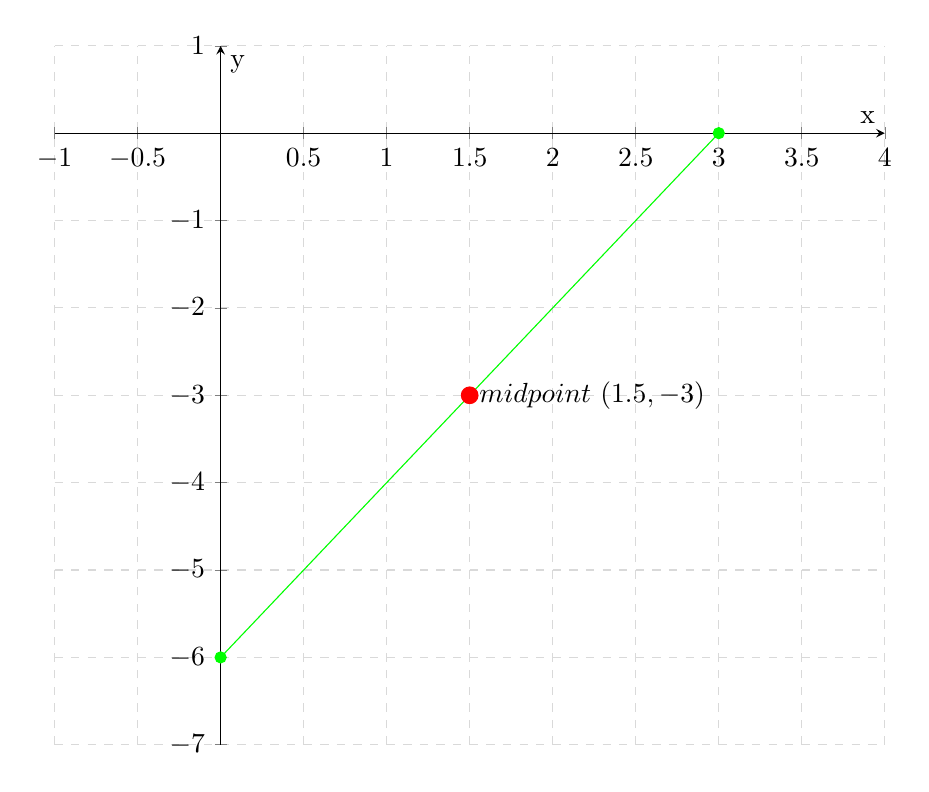
\begin{tikzpicture}
                    \begin{axis}[
                            width= \linewidth,
                            xmin = -1,
                            xmax = 4,
                            ymin=-7,
                            ymax=1,
                            xlabel=x,
                            ylabel=y,
                            grid=major,
                            grid style = {dashed, gray!30},
                            axis lines = center,
                            clip = false
                        ]

                        \addplot[color=green,mark=*] coordinates {
                                (0, -6)
                                (3, 0)
                            };

                        \addplot[color=red, mark=*, mark size=3pt] coordinates {
                                (1.5, -3)
                            };

                        \node [right] at (axis cs: 1.5, -3) {$midpoint \ (1.5, -3)$};

                    \end{axis}
                \end{tikzpicture}
                \caption{\label{Graph-3}Graph showing $y=2x-6$}
            \end{center}
        \end{figure}
        \clearpage
        \subsection{(1, -7),(9, 0)}
        \underline{MIDPOINT}
        $$
            \begin{aligned}
                midpoint & = (\frac{x_1+x_2}{2}, \frac{y_1+y_2}{2}) \\
                         & = (\frac{1+9}{2}, \frac{-7+0}{2})        \\
                         & = (\frac{10}{2}, \frac{-7}{2})           \\
                         & = (5, -3.5)                              \\
            \end{aligned}
        $$

        \underline{LENGTH OF LINE}
        $$
            \begin{aligned}
                length \ of \ line & = \sqrt{(x_2-x_1)^2 + (y_2-y_1)^2} \\
                                   & = \sqrt{(9-1)^2 + (0-(-7))^2}      \\
                                   & = \sqrt{(8)^2 + (7)^2}             \\
                                   & = \sqrt{64 + 49}                   \\
                                   & = \sqrt{113}                       \\
                                   & = 10.63                            \\
            \end{aligned}
        $$

        \underline{SLOPE OF LINE}
        $$
            \begin{aligned}
                m & = \frac{y_2-y_1}{x_2-x_1} \\
                  & = \frac{0-(-7)}{9-1}      \\
                  & = \frac{7}{8}             \\
                  & = 0.88                    \\
            \end{aligned}
        $$

        \underline{EQUATION OF THE LINE}

        Using the points $(1, -7)$ and $m=0.88$ we find $c$
        $$
            \begin{aligned}
                y & = mx + c       \\
                c & = y - mx       \\
                c & = -7 - 0.88(1) \\
                c & = -7-0.88      \\
                c & = -7.88        \\
            \end{aligned}
        $$
        Therefore the equation is
        $$
            y = 0.88x-7.88
        $$
        \begin{figure}[H]
            \begin{center}
                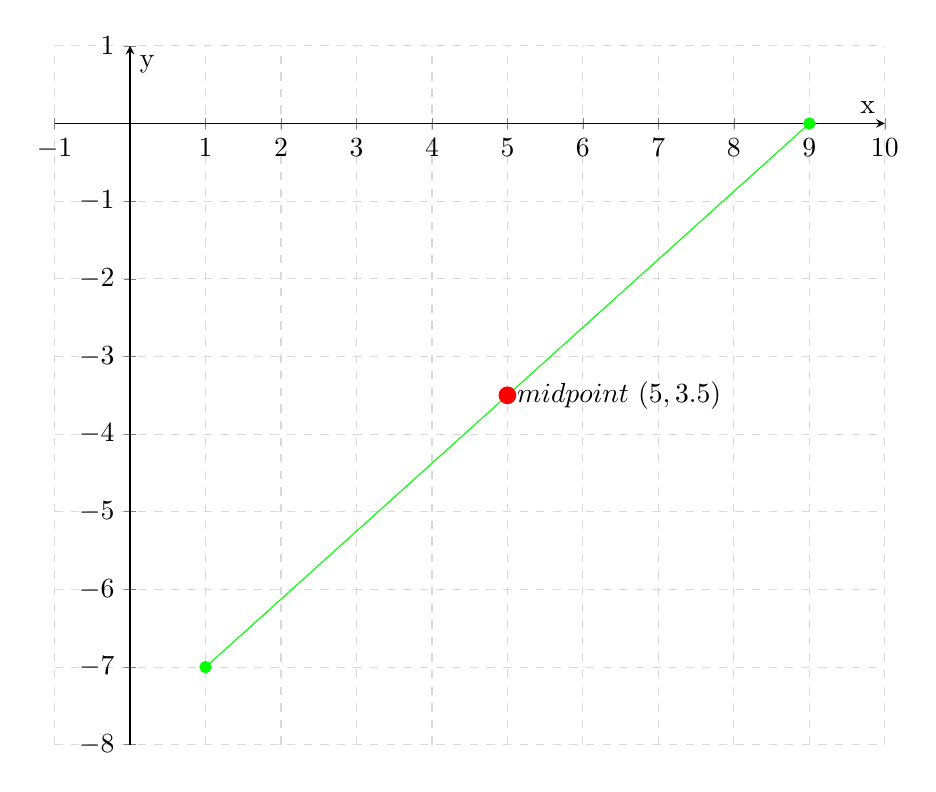
\begin{tikzpicture}
                    \begin{axis}[
                            width= \linewidth,
                            xmin = -1,
                            xmax = 10,
                            ymin=-8,
                            ymax=1,
                            xlabel=x,
                            ylabel=y,
                            grid=major,
                            grid style = {dashed, gray!30},
                            axis lines = center,
                            clip = false
                        ]

                        \addplot[color=green,mark=*] coordinates {
                                (1, -7)
                                (9, 0)
                            };

                        \addplot[color=red, mark=*, mark size=3pt] coordinates {
                                (5, -3.5)
                            };

                        \node [right] at (axis cs: 5, -3.5) {$midpoint \ (5, 3.5)$};

                    \end{axis}
                \end{tikzpicture}
                \caption{\label{Graph-4}Graph showing $y = 0.88x-7.88$}

            \end{center}
        \end{figure}
        \clearpage
        \subsection{(0, 9),(5, -6)}
        \underline{MIDPOINT}
        $$
            \begin{aligned}
                midpoint & = (\frac{x_1+x_2}{2}, \frac{y_1+y_2}{2}) \\
                         & = (\frac{0+5}{2}, \frac{9-6}{2})         \\
                         & = (\frac{5}{2}, \frac{3}{2})             \\
                         & = (2.5, 1.5)                             \\
            \end{aligned}
        $$

        \underline{LENGTH OF LINE}
        $$
            \begin{aligned}
                length \ of \ line & = \sqrt{(x_2-x_1)^2 + (y_2-y_1)^2} \\
                                   & = \sqrt{(5-0)^2 + (-6-9)^2}        \\
                                   & = \sqrt{(5)^2 + (-15)^2}           \\
                                   & = \sqrt{25 + 225}                  \\
                                   & = \sqrt{250}                       \\
                                   & = 15.81                            \\
            \end{aligned}
        $$

        \underline{SLOPE OF LINE}
        $$
            \begin{aligned}
                m & = \frac{y_2-y_1}{x_2-x_1} \\
                  & = \frac{-6-9}{5-0}        \\
                  & = \frac{-15}{5}           \\
                  & = -3                      \\
            \end{aligned}
        $$

        \underline{EQUATION OF THE LINE}

        Using the points $(0, 9)$ and $m=-3$ we find $c$
        $$
            \begin{aligned}
                y & = mx + c      \\
                c & = y - mx      \\
                c & = 9 - (-3)(0) \\
                c & = 9 - 0       \\
                c & = 9           \\
            \end{aligned}
        $$
        Therefore the equation is
        $$
            y = -3x + 9
        $$
        \begin{figure}[H]
            \begin{center}
                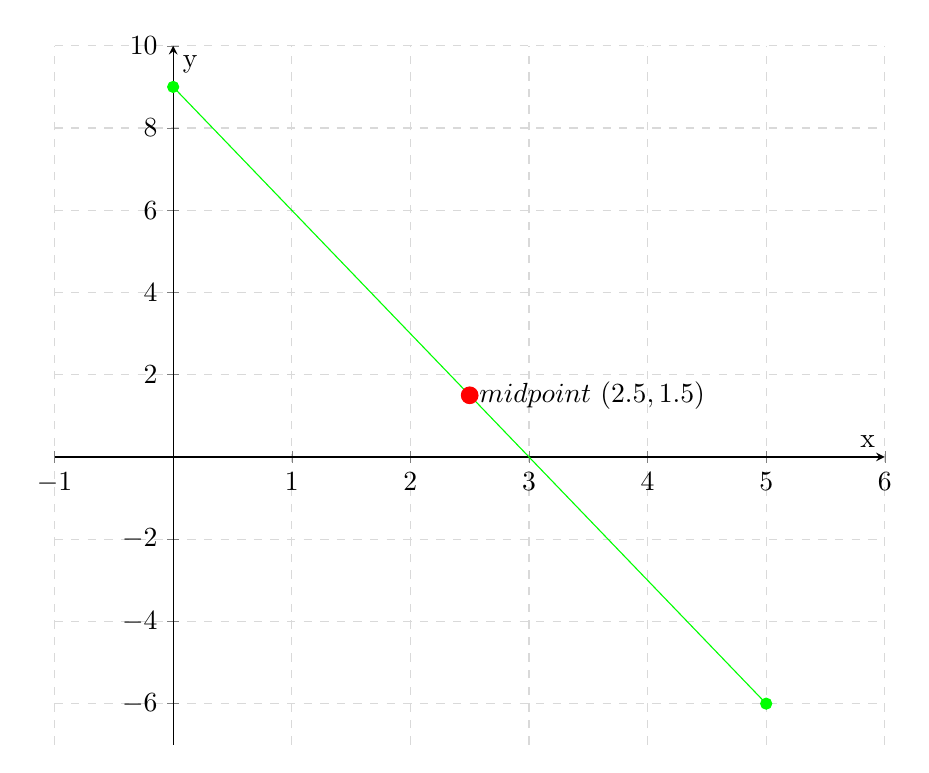
\begin{tikzpicture}
                    \begin{axis}[
                            width= \linewidth,
                            xmin = -1,
                            xmax = 6,
                            ymin=-7,
                            ymax=10,
                            xlabel=x,
                            ylabel=y,
                            grid=major,
                            grid style = {dashed, gray!30},
                            axis lines = center,
                            clip = false
                        ]

                        \addplot[color=green,mark=*] coordinates {
                                (0, 9)
                                (5, -6)
                            };

                        \addplot[color=red, mark=*, mark size=3pt] coordinates {
                                (2.5, 1.5)
                            };

                        \node [right] at (axis cs: 2.5, 1.5) {$midpoint \ (2.5, 1.5)$};

                    \end{axis}
                \end{tikzpicture}
                \caption{\label{Graph-5}Graph showing $y = -3x+9$}

            \end{center}
        \end{figure}
        \clearpage
        \subsection{(5, -2),(4,-2)}
        \underline{MIDPOINT}
        $$
            \begin{aligned}
                midpoint & = (\frac{x_1+x_2}{2}, \frac{y_1+y_2}{2}) \\
                         & = (\frac{5+4}{2}, \frac{-2-2}{2})        \\
                         & = (\frac{9}{2}, \frac{-4}{2})            \\
                         & = (4,5, -2)                              \\
            \end{aligned}
        $$

        \underline{LENGTH OF LINE}
        $$
            \begin{aligned}
                length \ of \ line & = \sqrt{(x_2-x_1)^2 + (y_2-y_1)^2} \\
                                   & = \sqrt{(4-5)^2 + (-2-(-2))^2}     \\
                                   & = \sqrt{(-1)^2 + (0)^2}            \\
                                   & = \sqrt{1+0}                       \\
                                   & = \sqrt{1}                         \\
                                   & = 1                                \\
            \end{aligned}
        $$

        \underline{SLOPE OF LINE}
        $$
            \begin{aligned}
                m & = \frac{y_2-y_1}{x_2-x_1} \\
                  & = \frac{-2-(-2)}{4-5}     \\
                  & = \frac{0}{-1}            \\
                  & = 0                       \\
            \end{aligned}
        $$

        \underline{EQUATION OF THE LINE}

        Using the points $(5, -2)$ and $m=0$ we find $c$
        $$
            \begin{aligned}
                y & = mx + c     \\
                c & = y - mx     \\
                c & = -2 -(0)(5) \\
                c & = -2 - 0     \\
                c & = -2         \\
            \end{aligned}
        $$
        Therefore the equation is
        $$
            y = -2
        $$
        \begin{figure}[H]
            \begin{center}
                \begin{tikzpicture}
                    \begin{axis}[
                            width= \linewidth,
                            xmin = 3,
                            xmax = 6,
                            ymin=-3,
                            ymax=0,
                            xlabel=x,
                            ylabel=y,
                            grid=major,
                            grid style = {dashed, gray!30},
                            axis lines = center,
                            clip = false
                        ]

                        \addplot[color=green,mark=*] coordinates {
                                (5, -2)
                                (4, -2)
                            };

                        \addplot[color=red, mark=*, mark size=3pt] coordinates {
                                (4.5, -2)
                            };

                        \node [right] at (axis cs: 4.5, -1.9) {$midpoint \ (4.5, -2)$};

                    \end{axis}
                \end{tikzpicture}
                \caption{\label{Graph-6}Graph showing $y = -2$}

            \end{center}
        \end{figure}
        \clearpage
\end{description}

\section{}
\subsection{Refer to the above, determine the equation of the line that is parallel to \hyperref[subsection:1.1]{(1.1)} but passes through (3, -2)}

Given the equation of line with points $(-2, 10),(5, 3)$ i.e. $A$ is
$$
    y = -x + 8
$$
The $y-intercept$ i.e. $c$ of line parallel to $A$ is
$$
    \begin{aligned}
        -2 & = -3 + c \\
        c  & = -2 + 3 \\
        c  & = 1      \\
    \end{aligned}
$$
Therefore the equation of the parallel line $B$ is
$$
    y = -x + 1
$$

\subsection{Determine the equation of the line that is perpendicular to \hyperref[subsection:1.1]{(1.1)} bit passes through (10, 3)}

Given the equation of line $A$ with points $(-2, 10),(5, 3)$ is

$$
    y = -x + 8
$$
and
$$
    m_1 = -1
$$
and two lines are $\perp$ when
$$
    m_1 * m_2 = -1
$$
$m_2$ is therefore
$$
    \begin{aligned}
        -1*m_2 & = -1            \\
        m_2    & = \frac{-1}{-1} \\
        m_2    & = 1             \\
    \end{aligned}
$$
The $y-intercept$ i.e. c of $\perp$ line $C$ using points $(10, 3)$ and $m=1$ is
$$
    \begin{aligned}
        y & = mx + c    \\
        3 & = 1(10) + c \\
        c & = -7        \\
    \end{aligned}
$$
Therefore the equation of $\perp$ line $C$ is
$$
    y = x-7
$$
\begin{figure}[H]
    \begin{center}
        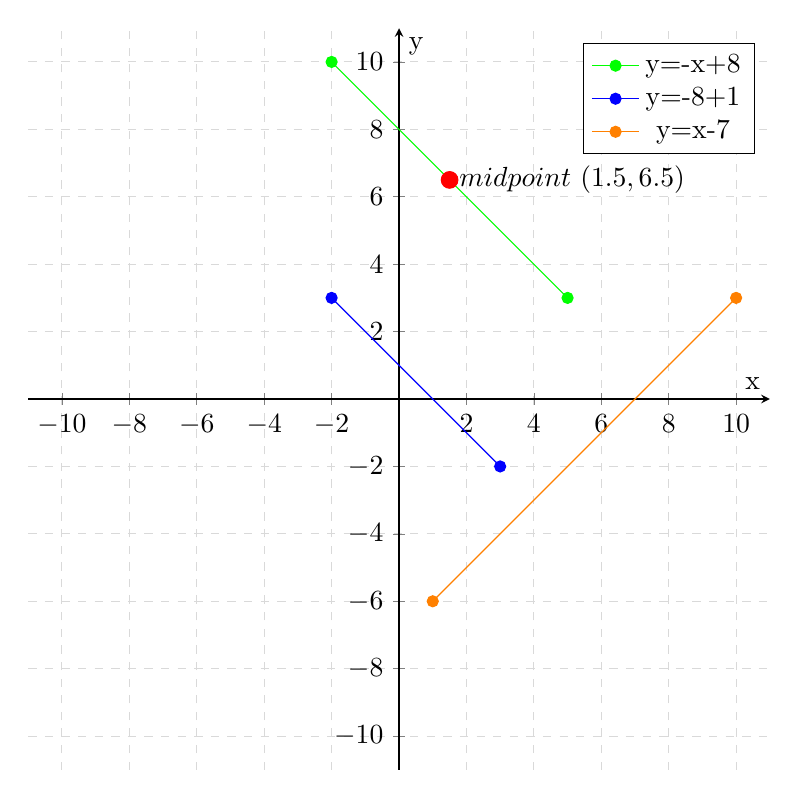
\begin{tikzpicture}
            \begin{axis}[
                    width = 11cm,
                    height= 11cm,
                    xmin = -11,
                    xmax = 11,
                    ymin=-11,
                    ymax=11,
                    xlabel=x,
                    ylabel=y,
                    grid=major,
                    grid style = {dashed, gray!30},
                    axis lines = center,
                    clip = false
                ]

                \addplot[color=green,mark=*] coordinates {
                        (-2, 10)
                        (5, 3)
                    };
                \addplot[color=blue, mark=*] coordinates {
                        (3, -2)
                        (-2, 3)
                    };

                \addplot[color=orange, mark=*] coordinates {
                        (10, 3)
                        (1, -6)
                    };
                \addplot[color=red, mark=*, mark size=3pt] coordinates {
                        (1.5, 6.5)
                    };

                \node [right] at (axis cs: 1.5, 6.5) {$midpoint \ (1.5, 6.5)$};

                \legend{y=-x+8, y=-8+1, y=x-7}

            \end{axis}
        \end{tikzpicture}
        \caption{\label{Graph-7}}
    \end{center}
\end{figure}
\clearpage

\section{Two points on a straight line are $P(6, 10)$ and $Q(-4, -6)$. Determine:}
\begin{description}
    \item[a.] the length of the line $PQ$
        $$
            \begin{aligned}
                 & = sqrt{(x_2 - x_1)^2 + (y_2-y_1)^2} \\
                 & = sqrt{(-4-6)^2 + (-6-10)^2}        \\
                 & = sqrt{100+156}                     \\
                 & = sqrt{256}                         \\
                 & = 18.87                             \\
            \end{aligned}
        $$
    \item[b.] the midpoint of $PQ$
        $$
            \begin{aligned}
                 & = (\frac{x_1+x_2}{2}, \frac{y_1+y_2}{2}) \\
                 & = (\frac{6-4}{2}, \frac{10-6}{2})        \\
                 & = (\frac{2}{2}, \frac{}{2})              \\
                 & = (1, 2)                                 \\
            \end{aligned}
        $$
    \item[c.] the equation of $PQ$
        The equation of a line is
        $$
            y = mx+c
        $$
        The slope of the line $PQ$ is
        $$
            \begin{aligned}
                m & = \frac{y_2-y_1}{x_2-x_1} \\
                  & = \frac{-6-10}{-4-6}      \\
                  & = \frac{-16}{-10}         \\
                  & = 1.6                     \\
            \end{aligned}
        $$
        The $y-intercept$ of the line is
        $$
            \begin{aligned}
                c & = y - mx        \\
                c & = 10 - (1.6)(6) \\
                c & = 10 - 9.6      \\
                c & = 0.4           \\
            \end{aligned}
        $$
        Therfore the equation of the line is
        $$
            y = 1.6x + 0.4
        $$
    \item[d.] the equation of the line $MN$ that is $\parallel$ to $PQ$ and passes through $(0, -8)$
        Given that MN $\parallel$ to PQ
        $$
            m = 1.6
        $$
        The intercept of the line $MN$ is using the points $(0,-8)$ is
        $$
            \begin{aligned}
                y  & = 1.6x + c   \\
                -8 & = 1.6(0) + c \\
                c  & = -8         \\
            \end{aligned}
        $$
        Therefore the equation of the line $MN$ is
        $$
            y = 1.6x-8
        $$
    \item[e.] the equation of the line $AB$ that is $\perp$ to $PQ$ but passes through $(10, 4)$
        Given $AB \perp PQ$, the slope of AB is
        $$
            \begin{aligned}
                m_1 * m_2 & = -1             \\
                1.6* m_2  & = -1             \\
                m_2       & = \frac{-1}{1.6} \\
                m_2       & = -0.625
            \end{aligned}
        $$
        The intercept of the line using the points $(10, 4)$ is
        $$
            \begin{aligned}
                c & = y - mx           \\
                c & = 4 - (-0.625)(10) \\
                c & = 4 - (-0.625)(10) \\
                c & = 4 + 6.25)        \\
                c & = 10.25)           \\
            \end{aligned}
        $$
        Therefore the equation of the line is
        $$
            y = -0.625x+10.25
        $$
\end{description}
\begin{figure}[H]
    \begin{center}
        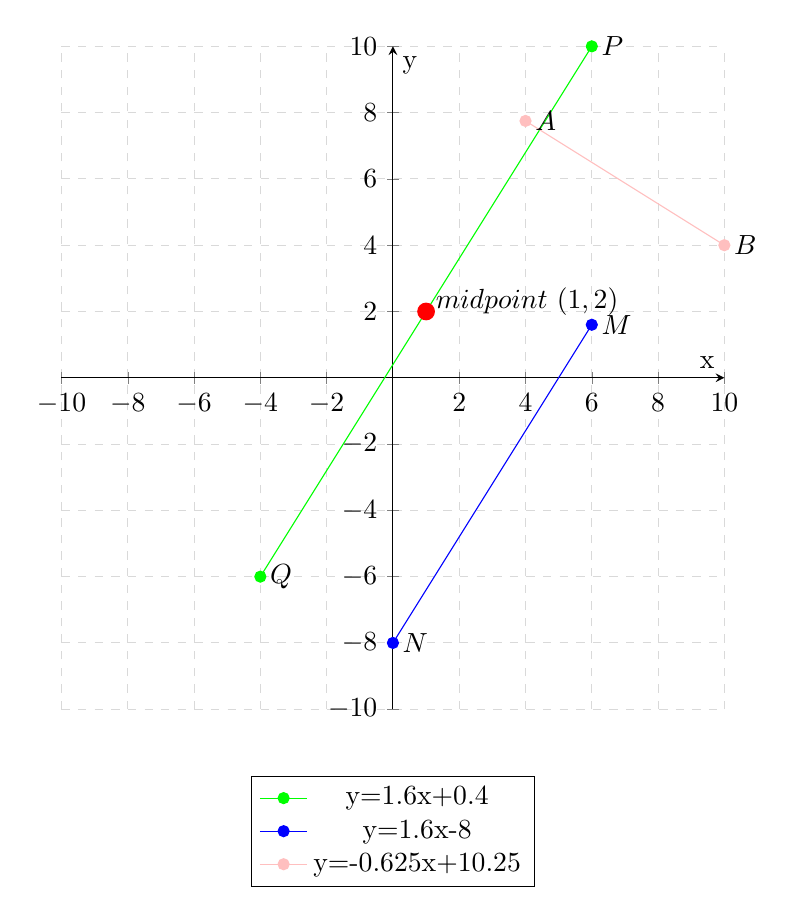
\begin{tikzpicture}
            \begin{axis}[
                    height=10cm,
                    width=10cm,
                    xmin = -10,
                    xmax = 10,
                    ymin=-10,
                    ymax=10,
                    xlabel=x,
                    ylabel=y,
                    grid=major,
                    grid style = {dashed, gray!30},
                    axis lines = center,
                    clip = false,
                    legend style={at={(0.5, -0.1)}, anchor = north}
                ]

                \addplot[color=green,mark=*] coordinates {
                        (6, 10)
                        (-4, -6)
                    };
                \addplot[color=blue,mark=*] coordinates {
                        (0, -8)
                        (6, 1.6)
                    };
                \addplot[color=pink,mark=*] coordinates {
                        (10, 4)
                        (4, 7.75)
                    };
                \addplot[color=red, mark=*, mark size=3pt] coordinates {
                        (1, 2)
                    };

                \node [right] at (axis cs: 1, 2.3) {$midpoint \ (1, 2)$};
                \node [right] at (axis cs: 6, 10) {$P$};
                \node [right] at (axis cs: -4, -6) {$Q$};
                \node [right] at (axis cs: 6, 1.6) {$M$};
                \node [right] at (axis cs: 0, -8) {$N$};
                \node [right] at (axis cs: 4, 7.75) {$A$};
                \node [right] at (axis cs: 10, 4) {$B$};

                \legend{y=1.6x+0.4,y=1.6x-8, y=-0.625x+10.25}

            \end{axis}
        \end{tikzpicture}
        \caption{\label{Graph-8}}
    \end{center}
\end{figure}
\clearpage
\subfile{sections/section_4}
\end{document}